\section{The Algorithms}\label{sec:the-algorithms}

\subsection{\texorpdfstring{$\halfMMS$}{1/2MMS} Indivisible Algorithm}\label{subsec:alg-indivisible}

This algorithm i will not implement myself, as i will utilize a already implemented algorithm\cite{Allocations} for $\halfMMS$ under works by \emph{Hummel} and \emph{Hetland}. This specific implementation has the additional specification of handling cardinality constraints.When i am using the algorithm i will not be utelizing these constraints by simply setting the constraint for all items to be the same as the total number of items. As the main benfit of using a already established algorithm is that there isn't such a need to understand all the details of the algorithm, as such i won't go into exact details of this algorithm here, and instead refer to the source directly for more details\cite{Allocations}.




\subsection{\texorpdfstring{$\halfMMS$}{1/2MMS} Indivisible Algorithm, Cut Cake in \texorpdfstring{$\sNumAgents$}{n} Pieces}\label{subsec:alg-cut-cake}

This isn't exactly a new algorithm, but for simplicity i will name it as such. This "algorithm" simply uses the algorithm from \autoref{subsec:alg-indivisible}, with the only difference being that there is now a small pre-processing step where the cake is cut into $\sNumAgents$ equal pieces, where $\sNumAgents$ is the number of agents. 

Take for instance the following matrix of valuations for three agents and two goods (one item and one cake). Each row represents an agent, and each column represents a good, where the final column is the cake. The conversion then looks like this:
$$
    \begin{bmatrix}
        1 & 1 \\
        2 & 2 \\
        3 & 3
    \end{bmatrix}
    \overset{\text{cut cake}}{\rightarrow}
    \begin{bmatrix}
        1 & 1/3 & 1/3 & 1/3 \\
        2 & 2/3 & 2/3 & 2/3 \\
        3 & 3/3 & 3/3 & 3/3
    \end{bmatrix}
$$
The algorithm then uses this new instance, and after the algorithm is completed a post processing step of gathering up these pieces again is performed by simply adding together $1/\sNumAgents$ per piece of cake an agent gets.

A conversion for a fair allocation of the instance above could look like this, the matrix show the allocation by having values from 0 to 1, which for items means they are either allocated to that agent or not. When converting back, since we know which rows correspond to pieces of cake, we simply add these pieces together to find how much of that cake is allocated to that agent in total.
$$
    \begin{bmatrix}
        0 & 0 & 1 & 1 \\
        0 & 1 & 0 & 0 \\
        1 & 0 & 0 & 0
    \end{bmatrix}
    \overset{\text{gather pieces}}{\rightarrow}
    \begin{bmatrix}
        0 & 2/3 \\
        0 & 1/3 \\
        1 & 0
    \end{bmatrix}
$$
To find the value each agent has for their bundle these values can they simply perform element-wise multiplication of the allocation matrix and the valuation matrix, and sum the rows. This gives the following result:
$$
    \begin{bmatrix}
        0 & 2/3 \\
        0 & 1/3 \\
        1 & 0
    \end{bmatrix}
    \cdot
    \begin{bmatrix}
        1 & 1 \\
        2 & 2 \\
        3 & 3
    \end{bmatrix}
    =
    \begin{bmatrix}
        0 & 2/3 \\
        0 & 2/3 \\
        3 & 0
    \end{bmatrix}
    \rightarrow
    \begin{bmatrix}
        2/3 \\
        2/3 \\
        3
    \end{bmatrix}
$$
A consequence of the cake cutting is that the size of the instance increases by $\sNumAgents$ items per cake. This will have a negative impact on the running time of the algorithm. This is also why, in an attempt to "mimic" a divisible good, cutting a cake into as tiny pieces as possible isn't a viable strategy. 







\subsection{\texorpdfstring{$\halfMMS$}{1/2MMS} Mixed Algorithm}\label{subsec:alg-mixed}

This is an implementation of the Half-MMS Algorithm for Homogenous Cake described by \emph{Bei et al.}\cite{mixed-goods}. For completeness the pseudocode for the algorithm is shown in \autoref{alg:mixed}. The algorithm is split into two main phases.

\subsubsection{Phase 1: Large Items}
Initially any item $\sItem$ worth more than $\halfMMS_\sAgent$ for any agent $\sAgent$ are allocated to that agent. This is done until no more such items exists in the instance. Each agent (and of course the item) is then removed from any further consideration. See while loop from line \ref{line:mixed-phase1} in \autoref{alg:mixed}.

\subsubsection{Phase 2: Small Items and Cake}
Next an empty bundle $B$ is initialized. A small item (width less than $\halfMMS_\sAgent$) is then added to the bundle and each agent looks at this item, and figures out how much cake they would need in addition to this item in order to achieve a total valuation of $\halfMMS_\sAgent$ for the bundle, formally $\sValuation_\sAgent(\sBundle) + x\sValuation_\sAgent(\sTheCake) == \halfMMS_\sAgent$. This bundle, and that amount of cake is then allocated to the agent that required the \emph{least} amount of cake. This repeats until either all items are gone, or all agents have received their $\halfMMS_\sAgent$. See while loop from line \ref{line:mixed-phase2} in \autoref{alg:mixed}.

Finally any remaining items or cake is allocated by using bag-filling to the last agent.

\begin{algorithm}
    \caption{Mixed-MMS-Homogenous}\label{alg:mixed}
    \begin{algorithmic}[1]
        \Require Agents $\sAllAgents$, indivisible goods $\sAllItems$ and a homogenous cake $\sTheCake$ and Valuation Functions $\sAllValuations$.
        \State Compute $\MMS_\sAgent$, for each $\sAgent\in\sAllAgents$.
        \State $\sBundle_1, \sBundle_2, ...,\sBundle_\sNumAgents\gets\emptyset$
        \While{$\exists\sAgent\in\sAllAgents, \sItem\in\sAllItems$ s.t. $\sValuation_\sAgent(\sItem) \geq \halfMMS_\sAgent$}\label{line:mixed-phase1}
            \State $\sBundle_\sAgent\gets\{\sItem\}$
            \State $\sAllAgents\gets\sAllAgents\backslash\{\sAgent\}$
            \State $\sAllItems\gets\sAllItems\backslash\{\sItem\}$
        \EndWhile
        \While{$\sNumAgents\geq2$}\label{line:mixed-phase2}
            \State $\sBundle\gets\emptyset$
            \State Add one item to $B$ until $\exists\sAgent\in\sAllAgents,\sValuation_\sAgent(\sBundle) \geq\halfMMS_\sAgent$ or $\sBundle=\sAllItems$.
            \State For each $\sAgent\in\sAllAgents$ set $x_\sAgent$ s.t. $\sValuation_\sAgent(\sBundle\cup\sTheCake_{x_\sAgent}) \geq \halfMMS_\sAgent$.
            \State $\sAgent^*\gets\arg\min_{\sAgent\in\sAllAgents}x_\sAgent$
            \State $\sBundle_{\sAgent^*}\gets\sBundle\cup\sTheCake_x$
            \State $\sAllAgents\gets\sAllAgents\backslash\{\sAgent^*\}$
            \State $\sAllItems\gets\sAllItems\backslash\sBundle$
            \State $\sTheCake\gets\sTheCake\backslash\sTheCake_x$
        \EndWhile
        \State Give all remaining items to last agent.\label{line:mixed-phase3}
        \State \Return $\{\sBundle_1, \sBundle_2, ...,\sBundle_\sNumAgents\}$
    \end{algorithmic}
\end{algorithm}





\subsection{Visualized Allocations}

In order to visually distinguish how these three variations of the algorithms work, more specifically how they handle the cake, i included \autoref{fig:allocations}. The stacked bars show how each agent values each bundle in the allocation, so both their own bundle, and the others bundle (semi-transparent). The dashed black line shows $\MMS_\sAgent$ for that agent $\sAgent\in\{1,2,3\}$, and the red dashed line is $\halfMMS_\sAgent$. See \autoref{fig:allocation_all_mms} to see exactly how each agent achieves this $\MMS$. The goal for the algorithms is then to allocate the goods such that the value each agent gives their own bundle crosses the red dashed line.

\begin{figure}
    \centering
    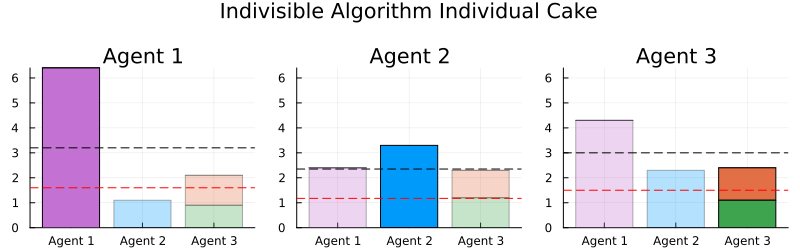
\includegraphics[width=\textwidth]{allocation_indivisible.png}
    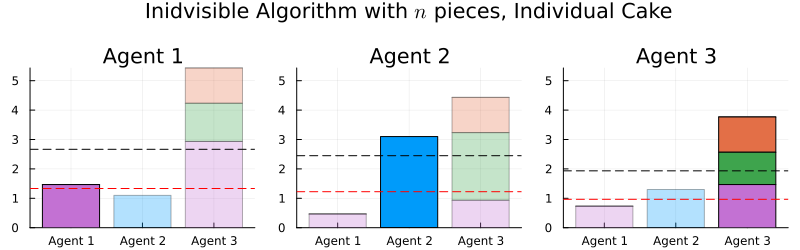
\includegraphics[width=\textwidth]{allocation_n_pieces.png}
    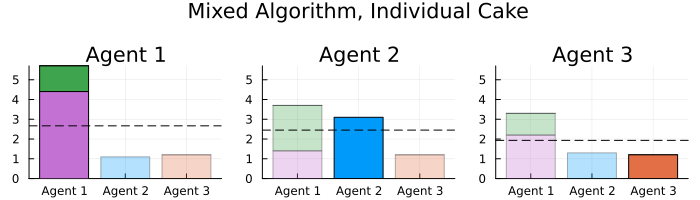
\includegraphics[width=\textwidth]{allocation_mixed.png}
    \caption{Result of the three main algorithms on the same instance with Individual Cake from \autoref{sec:preliminaries}.}
    \label{fig:allocations}
\end{figure}

For instance if we look at the top left chart, which is how Agent 1 sees the allocation after using the Indivisible algorithm. Agent 1 receives well over their expected MMS value, and Agent 1 is not envious of any other agent as the other agents bundles (semi-transparent) are all lower than their bundle. We also see (unsurprisingly) that the indivisible algorithm doesn't divide the cake, while the after cutting the cake into 3 pieces, the same algorithm gives 1 piece of cake to agent 1, and 2 pieces to agent 3. Finally the mixed algorithm gives just enough cake to agent 3 for agent three to receive $\frac{1}{2}\MMS_3$, and then gives the rest of the cake to agent 1.